\documentclass[12pt]{article}
%Required: You must have these
\usepackage{graphicx}
\usepackage{tabularx}
\usepackage{natbib}
\usepackage{lineno}
\linenumbers

\usepackage{array}
\usepackage{amsmath}
%\usepackage[backend=bibtex]{biblatex}
\setkeys{Gin}{width=0.8\textwidth}
%\setlength{\captionmargin}{30pt}
\setlength{\abovecaptionskip}{10pt}
\setlength{\belowcaptionskip}{10pt}
 \topmargin -1.5cm 
 \oddsidemargin -0.04cm 
 \evensidemargin -0.04cm 
 \textwidth 16.59cm
 \textheight 21.94cm 
 \parskip 7.2pt 
\renewcommand{\baselinestretch}{1.2} 	
\parindent 0pt

\bibliographystyle{..//..//refs/bibstyles/amnat.bst}
\usepackage{xr-hyper}
\usepackage{hyperref}


\title{
Exposure to frost risk across geographic ranges contributes to phenological cue differences among woody plants of temperate North America and Europe, but leaves much unexplained\\
Other
}

\author{Dan, Cat, Nacho, Ben Cook, Faith, Deidre, Mira Geoff and Lizzie}
\usepackage{Sweave}
\begin{document}
\Sconcordance{concordance:ranges_outline.tex:ranges_outline.Rnw:%
1 243 1 51 0}

\maketitle

\section*{Abstract}
\section*{Introduction}
New Outline Nov 2022:
\begin{enumerate}
\item Tradeoff between frost risk and growth shape phenological optimums
\item Frost risk varies
\item species evolve mechanisms to mitigate this risk
\item Species use different cues
\item cue differences result in more conservative strategies so in theory these should relate
\item this hasnt been super well tested
\subsection{Defining frost risk}
\item freeze risk is high when a) many gdds before last freeze event, and b) high interannual variation (ie last freeze is unpredicatble)
\subsection{Predictions for relationship between freeze risk and cues}
\item increased risk should rely on secondary cues/ and or more forcing.
\end{enumerate}


For woody plants at temperate latitudes, the phenology, or annual timing, of spring budburst influences a myriad of ecological processes including patterns of resource allocation \citep{Seiwa:1991vr}, trophic interactions \citep{Memmott2007} and biogeochemical cycling \citep{Piao2007}.
Through budburst timing, woody plants balance the advantages of precocious growth resumption for resource gains with the risk of damage from late season freezes \citep{Savage:2013aa}. 
To navigate this trade-off, woody plants have evolved complex physiological responses to sense environmental cues that signal the arrival of appropriate conditions for resuming growth \citep{}.

Yet frost risk varies a lot over space and time
%Frost risk


%Decades of research suggest that warming spring temperatures (forcing), cool winter temperatures (chilling) and day length (photoperiod) are primary environmental cues utilized by woody plants to determine the timing of spring phenological events \citep{Ettinger:2020aa,Forrest2010}. These studies also demonstrate the there are substantial cue-use differences among species, with some species relying more heavily on some cues over others \citep{Laube:2014aa,}. As anthropogenic climate change has already driven shifts in spring phenology \citep{Menzel2006}, identifying these inter-specific differences in cue use has emerged as a major goal of phenological research \citep{Chuine2002}. These differences have strong implications for both predicting the rate of phenological shifts as the climate continues to warm \citep{?}, and anticipating the ecological consequences of these shifts \citep{Cleland2012}. 

\noindent We leveraged over 50 years worth of phenology experiments in the OSPREE database \citep{wolkovich2019} and climate data collected across the ranges of temperate woody species in North America and Europe to assess X. We used a Bayesian hierarchical approach to jointly fit models estimating of forcing, chilling and photoperiod sensitivity for each species and the effects of the interannual variation in number of growing degree days before the last frost in species ranges on these estimates. Then for a subset of well represented species in our dataset, we modeled the among and within species variation in cue use to quantify the relative strength of local adaptation of pattern of phenological cue use. With this approach we 1) clarify the relationships between climatic variability across multiple scales of spatio-temporality, 2) identify the climate drivers that are more and less likely to drive selection on phenological cues and 3) compare variation in cue-use among and within species and between temperate Europe and North America. Our interrogation of these relationships between climate and cue use not only elucidates the evolutionary drivers of phenological cues, but offers new insights regarding implications of climate change as both species' ranges and phenology continue to shift with warming.


\section*{Methods}
%Dan and/or Lizzie write:
%\begin{itemize}
%\item Introduce OSPREE
%\item Species selection
%\item Model description
%\end{itemize}
\subsection*{OSPREE database}
To estimate phenological responses to chilling, forcing and photoperiod we used data from the Observed Spring Phenology Responses in Experimental Environments (OSPREE) database  \citep{wolkovich2019}. This database aims to include data from all published studies of experiments on woody plant responses to chilling, forcing and photoperiod cues, as described in \citet{Ettinger:2020aa}. Here we use a subset of data from a version of the database updated in June 2019, selecting species for which we could reliably estimate cue responses. As such, we included species that where: 1) included in two or more studies, 2) we had data for at least two levels of each cue (chilling, forcing and photoperiod; but we excluded species that only had field chilling), and 3) could obtain published range maps (see below). While this approach limited our total species number, it provided more reliable estimates of phenological cues (see Supplement). 

%EMWFeb5: Dan, can you move to supp (below text)? It could be a section where we include this text and perhaps more on the population model stuff. 
%EMWFeb5: Do we discuss anywhere the chilling issue for the pop model?
% Estimates of phenological cues (i.e., change in days of an event per change in level of chilling, forcing or photoperiod) can vary strongly due to study location and methodological differences (CITES). For example, many studies often include only one--often extreme---level of a cue, such as a photoperiod of 24 hours or very low chilling, and thus will provide estimated responses to the manipulated cues (e.g., forcing) relevant only in those extremes. Some statistical methods can estimate responses across such data, but they will estimate cue responses as more similar across all species than they likely are \citep[see][for example]{Ettinger:2020aa}, making the type of inter-specific comparisons we were interested in here difficult. 
% Lizzie says:
% Not sure if we need the sentences in [] ... take them out as you like. 
% Dan, can you skim https://github.com/lizzieinvancouver/ospree/issues/379 and make sure my methods above seem to accurate compared to what we wrote in that issue?
% I included the longer methods on the update in Nacho's pheno-phylo ms for now (since that ms uses almost all the data). 

\subsection*{Species' range characteristics and climate data}
%Cat and/or Nacho write?\\

We extracted climate data  from daily gridded meteorological datasets for both Europe and North America. For Europe, we extracted minimum and maximum daily temperatures from the E-OBS dataset (\url{https://cds.climate.copernicus.eu/cdsapp#!/dataset/insitu-gridded-observations-europe?tab=overview}; last accessed on October 2021) corresponding to the period comprised between 1980 and 2016. Specifically, we used version 17 at a resolution of 0.5 latitudinal degrees. For North America, we extracted minimum and maximum daily temperatures from Justin Sheffield's Princeton Global Forcing dataset (\url{http://hydrology.princeton.edu/data/pgf/v3/0.25deg/daily/}; last accessed on October 2021) for the same period. We used version v3 at a resolution of 0.25 latitudinal degrees. 

For 22 European and 16 North American tree species, we obtained published distributional range maps in shapefile format. European species ranges were downloaded from (\url{http://www.sciencedirect.com/science/article/pii/S2352340917301981?via\%3Dihub#ec-research-data}; last accessed on XXX) \citep{Caudullo2017} and North American ranges were obtained from \url{https://www.fs.fed.us/nrs/atlas/littlefia/#} \citep{Prasad2003}. For each species' range, we extracted climate data corresponding to all grid cells contained within the range.

We used minimum and maximum daily temperatures within species ranges were then used to compute Growing Degree Days (GDD), Growing Degree Days until the last frost (GDDlf) and Spring Temperature Variability (STV). GDD was calculated as the summed temperatures above 10$\degree$C recorded from January 1st until May 31st. GDDlf was calculated as GDD but instead of summing temperatures above a threshold until a fixed date, the sum was performed until the date at which the latest minimum temperature below -5$\degree$C was recorded. STV was calculated as the standard deviation of mean minimum temperature from March 1st until May 31st \citep{Zohner:2017aa}. Finally, as an additional metric of chilling we calculated chill portions \citep{?} using the daily minimum temperatures recorded each year from October 10th to February 28th. Because climate varies geographycally and temporally we calculated both the temporal and spatial variation in the above climate variables. Specifically, we computed the variability in the variables within each location across years (1980 to 2016) and for each year across the grid cells comprised within each species' range.
%\textbf{10th Oct - 28Feb (should be march to may)}. 
  

%IMCFeb21: I've tried the following: %\textbf{Some notes: can we add a sentence about temporal vs. spatial variation here? Also, we calculated Chill portions so we should include that here as well.} I do not remember the particular ref. we based our calculations of chill portions but can check in the ChillR package.


\subsection*{Statistical analysis}
\subsubsection*{Climate cue-use relationships}
To assess the relationships between range-wide climate variables and phenological sensitivity to forcing, chilling and photoperiod we fit Bayesian hierarchical phenology using a joint modeling framework in which we estimated all model parameters at once---both the phenological cues estimated from experiments and how range characteristics affected those cues. Traditionally, such modeling is done sequentially: first, estimating phenological cues in one more model, then using those estimated cues in a second model to estimate the relationship between cues and ranges. While simpler to fit, such models have the disadvantage of underestimating uncertainty (since it is rarely carried across models) and thus overestimating certainty and do not directly allow range effects to influence cue estimates since they are not estimated together. In contrast, our model yields parameter estimates where each cue response ($\beta_{chilling_{sp}}$, $\beta_{forcing_{sp}}$- and \beta_{photoperiod_{sp}}) is influenced by a range-wide climate variable  (via $ \beta_{trait x pheno}$ parameters) and can vary independently (via $\alpha_{forcing_{sp}$ ....) %EMWFeb5: Can you check and finish the math I started here (above)? 
The full model formulation is written below:\\

\begin{align*}
\hat{y}_{pheno, i} &= \alpha_{pheno, sp[i]} + \beta_{forcing_{sp[i]}}*F_i+\beta_{chilling_{sp[i]}}*C_i+\beta_{photoperiod_{sp[i]}}*P_i \\
\end{align*}
where:\\
\begin{align*}

\beta_{forcing_{sp}} & = \alpha_{forcing_{sp}} + \beta_{trait x pheno}*Variable_{climate} \\ %CJCFeb15: is this supposed to be `trait' here or is this carried over from the trait model syntax? 
\beta_{chilling_{sp}} & = \alpha_{chilling_{sp}} + \beta_{trait x pheno}*Variable_{climate} \\
\beta_{photoperiod_{sp}} & = \alpha_{photoperiod_{sp}} + \beta_{trait x pheno}*Variable_{climate} \\
\alpha_{pheno, sp} & \sim N(\mu_{\alpha, pheno}, \sigma_{\alpha, pheno}) \\
\alpha_{forcing_{sp}} & \sim N(\mu_{\alpha, forcing}, \sigma_{\alpha, forcing})\\
\alpha_{chilling_{sp}} & \sim N(\mu_{\alpha, chilling}, \sigma_{\alpha, chilling})\\
\alpha_{photoperiod_{sp}} & \sim N(\mu_{\alpha, photoperiod}, \sigma_{\alpha, photoperiod})\\
y_{pheno} & \sim N(\hat{y}_{pheno},\sigma^2_{y, pheno}) 

\end{align*}

For each climate variable of interest, we fit a model with all species and then, to better evaluate the differences among North American and European taxa, additional models for species from each continent separately. All versions of this model were fit in Stan \citep{Carpenter2017}(\texttt{www.mc-stan.org}) using weakly informative priors. We ran each model on 4 chain with 4000 iterations, with a 3000 iteration warm-up, for a total of 4000 sampling iterations per parameter. 

\subsubsection*{Intra vs. interspecific models}
To assess variation within and across sites, we designed a two-level, hierarchical model using data from the OSPREE database. We subset ted the studies to include only those that had multiple provenance locations. 
%CJC15Feb: Since chilling estimates were either from experimental chilling, from field chilling or a combination of both, we removed `chilling' as a predictor for this model since it correlated so strongly with provenance latitude and would result in nonidentifiability in our results. 

We used a Bayesian mixed-effects hierarchical model approach to analyze our data to best estimate the day of budburst. We fit a Gaussian distribution model using study, species and population as intercepts, forcing and photoperiod as predictors (fixed effects) and species nested within population (i.e., site) as modeled groups (random effects). The Bayesian model was fit using Stan modeling language \citep{Carpenter2017}(\texttt{www.mc-stan.org}), accessed via the \textit{rstan} package (version 2.15.1), version 2.3.1, in R \citep{R}, version 3.3.1, and was written as follows: 

% Lizzie says: 
% We just write out 'normal' (and gamma etc.) in the lab, it's much clearer so I changed that
% You can you & so the equations all align more -- they will align wherever you put the & so I usually put it before the = 
% See issue 420

\begin{align*}

y & \sim normal(\alpha_0 + \alpha_{study[i]} + \alpha_{sp[pop[i]]} +& \beta_{forcing_{sp[pop[i]]]}} + \beta_{photoperiod_{sp[pop[i]]}} + \epsilon_[i]} ) \\
\epsilon_i & \sim normal(0,\sigma_y) \\
\end{align*}
\noindent The $\alpha$ and each of the 5 $\beta$ coefficients were modeled at the study, species, population, or species and population level, as follows:
\begin{align*}

\alpha_{study} & \sim normal(\mu_{study}, \sigma_{study}) \\
\alpha_{sp[pop]} & \sim normal(\mu_{sp}, \sigma_{sp}) \\
\mu_{sp} & \sim normal(\mu_{pop}, \sigma_{pop}) \\
\beta_{forcing_{sp[pop]}} & \thicksim normal(\mu_{forcing_[sp]}, \sigma_{forcing_[sp]}) \\
\beta_{forcing_{sp}} & \thicksim normal(\mu_{forcing_[pop]}, \sigma_{forcing_[pop]}) \\
\beta_{photoperiod_{sp[pop]}} & \thicksim normal(\mu_{photoperiod_[sp]}, \sigma_{photoperiod_[sp]}) \\
\beta_{photoperiod_{sp}} s&  \thicksim normal(\mu_{photoperiod_[pop]}, \sigma_{photoperiod_[pop]}) \\

\end{align*}

We ran four chains, with 2,500 warm-up iterations followed by 3,000 sampling iterations, resulting in 12,000 posterior samples for each parameter. We assessed good model performance through $\hat{R}$ close to 1 and high $n_{eff}$ as well as visual consideration of chain convergence and posteriors \citep{Gelman2006}. Using the \textit{Gabry2017} package \citep{bayesplot}, we then plotted the partition of variance across the intercepts and predictors to determine intra- vs. inter-specific variation.  



\section*{Results}
%EMWFeb5: I like this! But, again, perhaps treat as an 'assumptions' section and thus present it first off *with* the pop models?
\subsection*{Coherence of spatio-temporal spring climate variability}
\textbf{I'd like to remove this as a full on ``result" and either put in in the methods sections to explain why we use one version of variation or elaborate on it in the suppliment but I am not so sure}
The spatio-temporal coherence of spring climate variability and intensity varied across continent and scales. Generally climate intensity (mean GDDs in range, mean Chill Portions in range, and Mean GDDs to last frost) were well correlated with climate variability (Fig. \ref{fig:corrs}) though strong differences can be observed between North America and Europe.  %Intra-annual, inter-annual and spatial variability in spring climate were also well correlated  (Fig. \ref{fig:corrs}e),f),g)), though the variability of spring climate in Europe was very low, suggesting that these correlation are likely more relevant in North America.
%IMCFeb21: again I wonder if we should talk about scales... not sure what a good alternative would be though, 'dimensions'?

\subsection*{Climate intensity and cue use}
%EMWFeb5: Can you work on saying things more biologically throughout results (for example. 'weak effects' is not as biological as it could be). 
%IMCFeb21: suggested edit - ...(Chill Portions) experienced within species' ranges did not seem to   associate with the sensitivity of those species to related cues. This is, the species that shift more their spring phenology as a response to forcing or chilling in experimental settings are not necessarily those with geographical ranges encompassing higher forcing or chilling average values. 
Overall, the mean forcing (GDDs) and chilling (Chill Portions) had weak effects on estimated cue-use. 
In our full species models mean GDDs had a weakly negative or neutral association with cue strength (GDD:Chill=X ,GDD:Force=Y, GDD:Photo=Z, (Fig. \ref{fig:mods1} a),b))). The general sign of these relationships persisted in the continent subset models (Fig. \ref{fig:mods1} d),e),f)) with the exception of the relationship between mean GDDs and chilling for North American species which became positive (mean= Z, (Fig. \ref{fig:mods1} c)). Generally, there was high uncertainty around these estimates.% suggesting climate intensity is a poor predictor for cue use. 



\subsection*{Climate variation and cue use}
In our full models, variation in growing degree days before the last frost of the season was weakly positively associated with forcing and photoperiod sensitivity and negatively associated with chilling sensitivity (Fig. \ref{fig:mods2}a))). However, our continent subset models show different effects. The effect of variation in GDDs to last frost (GDDlf) is poorly estimated in the European data subset,and has almost no effect on cue use over the narrow range of spring climate variation present in Europe  (Fig. \ref{fig:mods2}b). In contrast, in the North America subset, variation in GDDlf increases sensitivity in all three cues (Chilling:X Forcing:Y Photoperiod:Z, (Fig. \ref{fig:mods2}c))) suggesting there may be support for the climate variation hypotheses in North America where spring climate variation can be extreme. We found qualitatively similar continental patterns in the relationships between cue-use and climate variability using STV as an alternative metric inter-annual variation (see Supp).
%IMCFeb21: I may be reading the figure wrongly, but in Fig. 4 it seems like chilling has the positive correlation and forcing the negative one in panel A, doesn't it? Also, I would try to be more specific about what poorly estimated means (high uncertainty, all species get the same slopes, etc).


\subsection*{Cue use in North America and Europe}
%EMWFeb5: Do we explain the continent models in the methods? (I may have missed it, in which case, ignore me!)
We found that the strength of secondary cue use (chilling and photoperiod) was higher in North America than in Europe (Chilling: NA-X, EU-Y, Photoperiod NA-X, EU-Y, Fig.\ref{fig:cuediff}), while forcing sensitivity was higher in Europe than North America (NA-X, EU-Y). This result is consistent with the observation that the spring climate of North America is much less stable than Europe and our finding that the climate-cue use hypotheses appear to be better supported in North America.
%IMCFeb21: Perhaps we could cite Fig. 1 in support of the idea that spring climate is harsher in North America? 

\subsection*{Local adaptation of phenological cues}
We detected limited population level variation in forcing and photoperiod cue sensitivity, though this within species variation was less substantial than among species variation (Fig. \ref{fig:popy}). Notably, we found the largest source of variation in phenological cue estimates was the study effect Fig. \ref{fig:popy}).

\section*{Discussion}
\subsection*{Hypotheses of bioclimatic cue use} %IMCFeb21: why bioclimatic? If we go for this we should be consistent across. Also, perhaps we could make it clearer that when we talk about positive associations we mean between GDD and the absolute value of the sensitivity (looking at the figure, the negative slope of the sensitivity-GDD line can be misleading)
Similar to previous studies, we found stronger support for the climate variability hypothesis than the climate intensity hypothesis \citep{Zohner:2017aa}. While, as predicted by the climate intensity hypothesis, mean growing degree days in the range were positively associated with forcing sensitivity in North America, chilling sensitivity has no clear relationship with mean chilling in the range for species on either continent (Fig \ref{fig:mods1}e,f).  Further, there is high uncertainty surrounding the estimates in our climate intensity models, suggesting climate intensity is a poor predictor of phenological cue-use within species' ranges.

\noindent By contrast, climate variability was associated with increased forcing, chilling and photoperiod sensitivities in North American species (Fig \ref{fig:mods2},c) as predicted by the climate variability hypothesis. Interestingly, there was virtually no relationship between climate variability and cue-use in European species (Fig \ref{fig:mods2},b). We recovered these contrasting patterns among continents using multiple metrics of of climate variability (see Fig. S\ref{fig:STV}, and ``STV"). We also found secondary cue use (photoperiod and chilling) sensitivity was higher in North American taxa than in European ones (Fig. \ref{fig:cuediff}). These contrasting biological patterns appear to reflect the strong climatic differences we observed between the continents. %EMWFeb5:  Great paragraph

\subsection*{Climate patterns in North America and Europe}
Our study highlights that patterns of temperature variation and intensity are much stronger in temperate North America than in Europe (Fig. \ref{fig:concept}). This is a well established meteorological phenomenon driven by large local climate patterns like the jet stream and enso and stuff \textbf{(say better. maybe, Ben can write this paragraph)}. Additionally, we found that in North America, there was a strong correlation between temporal and spatial climatic variability across the geographic ranges of the species we studied, while in Europe this correlation was weakly negative. %IMCFeb21: perhaps add a citation to the corresponding figure in the supp?

%EMWFeb5: Lots of good stuff in paragraph below
\noindent When we consider our biological findings about cue-use differences among taxa in North America vs. Europe in the context of these climatic patterns, it is clear that this stark contrast must be better accounted for in understanding the evolutionary histories and ecological trajectories of the flora of these two continents. For any trait under selection, there must be sufficient selection pressure to drive the evolution of a trait \citep{}. Our results suggest that the recent magnitude of climate variation in Europe may be insufficient to drive the evolution of phenological sensitivity to climate cues. Additionally the lack of correlations we found between spatial and temporal climate variability in Europe could also suggest that the axes of variability could be muting selection.%CJCFeb15: Nice!! I like this paragraph a lot
\textbf{There is a known interaction of these forces in a some papers that Lizzie sent to Faith, so maybe we can explain and cite them here}. While previous work has suggested that climate variability drive cue use differences between North America and Europe \citep{Zohner:2017aa}, the absence of a relationship between climate variability and cue use we found in our European data subset, combined with the the weaker sensitivity to secondary cues, suggests a slightly different formulation. Our work suggests that climate variability may drive cue use only in North America where variation is sufficiently high to drive selection and not in Europe where variation is more limited. 

\noindeny While phenological data collected across Europe and North America are often utilized in tandem to test basic evolutionary and ecological theories, our finding supports the assertion of a growing number of researchers that given the differences in land use and geological history and contemporary and predicted climate change, that treating the flora of these two regions as discrete units may facilitate more nuanced understanding and precise predictions for temperate forest ecology ( I actually don't know if this is true). %EMWFeb5: Don't lump them together seems like a very good point, but I don't think treating them as 'discrete units' is the exact message we want either (though perhaps a good place to start, as we did). They're not entirely discrete units, but they must be analysed in a way that recognizes their different climatic and evolutionary histories. I would look at Cook et al. 2012 in Ecosystems and some Lechowicz work for what to say and cite. I like the point! We should keep it, but need to develop it. 
%IMCFeb21: I agree with Lizzie. Just to mention an author that has pushed that idea for long time, Ricklefs has a few papers where he advocates for separate analyses of taxa belonging to different biogeographical regions as they would have been subjected to differential 'regional effects': different histories of climate and other selective pressures at the biogeographic realm scale. While most of this literature is based on diversity, species richness and so on, some concepts would apply (I guess). I'm leaving here a couple refs in case they are useful:
%Latham, R. E., & Ricklefs, R. E. (1993). Continental comparisons of temperate-zone tree species diversity. Species diversity in ecological communities: historical and geographical perspectives, 294-314.
%Ricklefs, R. E., & He, F. (2016). Region effects influence local tree species diversity. Proceedings of the National Academy of Sciences, 113(3), 674-679.

\subsection*{Alternative hypotheses}

%EMWFeb5: The below feels like almost a final thought for the paper, I wondered if a new section might be better? Separate out more clearly assumptions we tested, versus alternatives still out there. I feel this section does a bit too much and yet never answers if not ranges, then what? I think we should discuss community differences (different leafout within one community) more somewhere in discussion. 
A major implication of our findings is the field of phenology must continue to expand the range of hypotheses we test and consider regarding the evolution of phenological cues. Phenology should continue to draw from studies of paleoclimate, biogeography, evolutionary ecology and community ecology. There is rich literature predicting that phenological cue differences among species may be the product of historic climate legacies \citep{}, strong phylogenetic constraints \citep{} or driven by community processes of phenological assembly like competition, niche theory  \citep{}. It is likely all of these factors along with the bio-climatic drivers we tested above drive selection on phenology and the the selection strength differs across time and space. Therefore, as we continue to gather more data on phenological cue use patterns for a more species, these hypotheses must be rigorously tested alongside the bio-climatic ones we address here.
%IMCFeb21: I wondered if, we could-should mention something about the implications of our results with respect the impacts of climate change on NAm vs Eur species. 

\noindent Additionally, while we found that species level variation in cue-use was higher than population level variation in our data, this finding was based on a limited subset of data because studies across many populations are rare. Further, we were unable to evaluate the level of local adaptation in chilling responses due to the way chilling treatments are most commonly applied \citep{}.\textbf{Maybe add a sentence explain why weinberger method doesn't allow for this}. There is a live debate surrounding the degree to which woody plant phenology is driven by local adaptation \citep{}, and phenological studies that contracts the responses of multiple populations are needed to understand these within species patterns. Importantly, when comparing the variation in population and species level phenological responses, we found that study effect to be significantly greater than either of these two axes of biological variation. (Maybe briefly elude to Zohner results here? but could cut if the new STV results are great. )

Increasing the geographic and taxonomic breadth of phenological cue experiments is critical to understanding the evolution of phenological cues, and predicting how these inter-specific differences in cues will impact forest ecology with global change. In both North America and Europe, the ranges of the species in our study we highly overlapping \textbf{(To do: make a mappy figure for supplement)}. It is possible that the influence of climate in range of species on differences in phenological cue use would be more pronounced for species with more discrete ranges (IE west vs. east coast of North America), but there is not currently enough taxonomic breadth in our phenological data to assess this. 

In this study we found limited support for the assertion that the climate variables that species encounter across their geographic ranges shape their relative reliance on forcing, chilling and photoperiod cues for spring phenology. Our results suggest that climate variability may drive cue use pattern only when it is sufficiently high, like in contemporary North America. These results suggests that future studies of phenological cue-use would benefit from a holistic integration of these bio-climatic hypotheses with phylogenetic, functional trait, and climatic legacy hypotheses to fully understand the evolution of phenological cues in woody plants, and how cue use patterns will impact species performance in the face of global change at across multiple spatial and temporal scales. %EMWFeb5:  Nice conclusion

\bibliography{..//..//refs/ranges}
\section*{Figures}

\begin{figure}[h!]
    \centering
 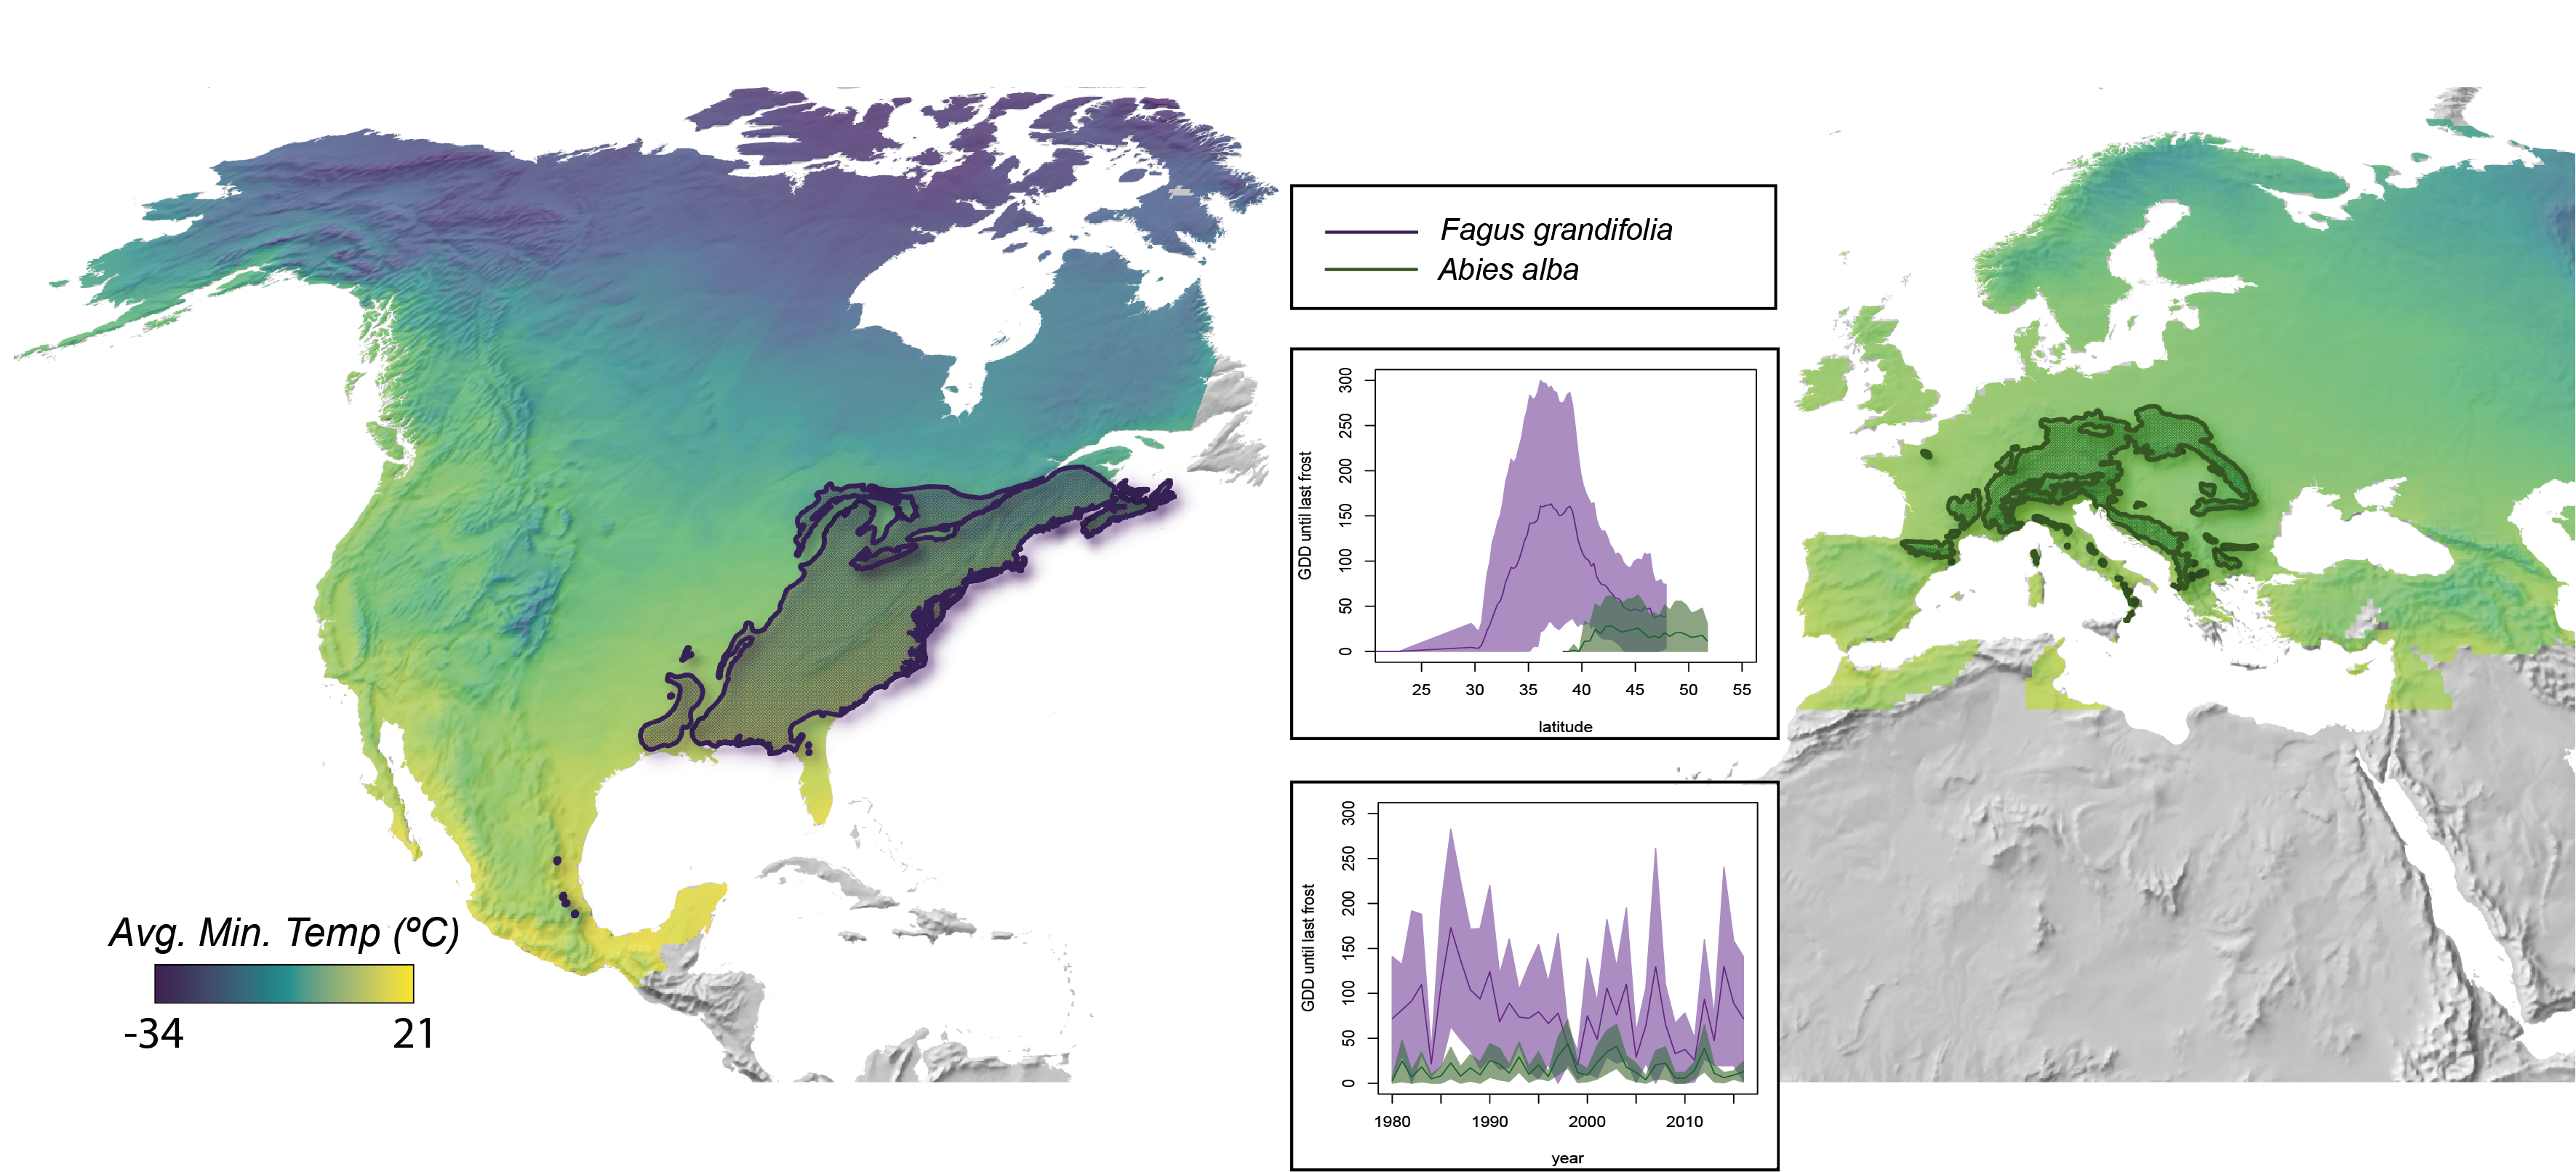
\includegraphics[width=\textwidth]{..//..//analyses/ranges/figures/concept figure draft2.png} 
    \caption{Illustration of the marked continental differences in spatial and temporal variation of climate within the geographic range of two example species: \emph{Fagus grandiflora} in purple and \emph{Abies alba} in green. The map shows the contrast between minimum temperatures averaged during winter across continents and how overlaid species' ranges may encompass different amount of variation in these temperatures. The insets show latitudinal (upper) and temporal (bottom) variation in Growing Degree Days recorded until the last day of frost (GDDlf) within each species range. It is to note that even if the European species' range reaches higher latitudes than the North American species, its climatic variation is sensibly smaller both temporally and spatially.}%Nacho, do you want to try taking a stab at this caption? I am happy to work on it if you want to start by just jotting a few notes/ideas down
    \label{fig:concept}
\end{figure}

\begin{figure}[h!]
    \centering
 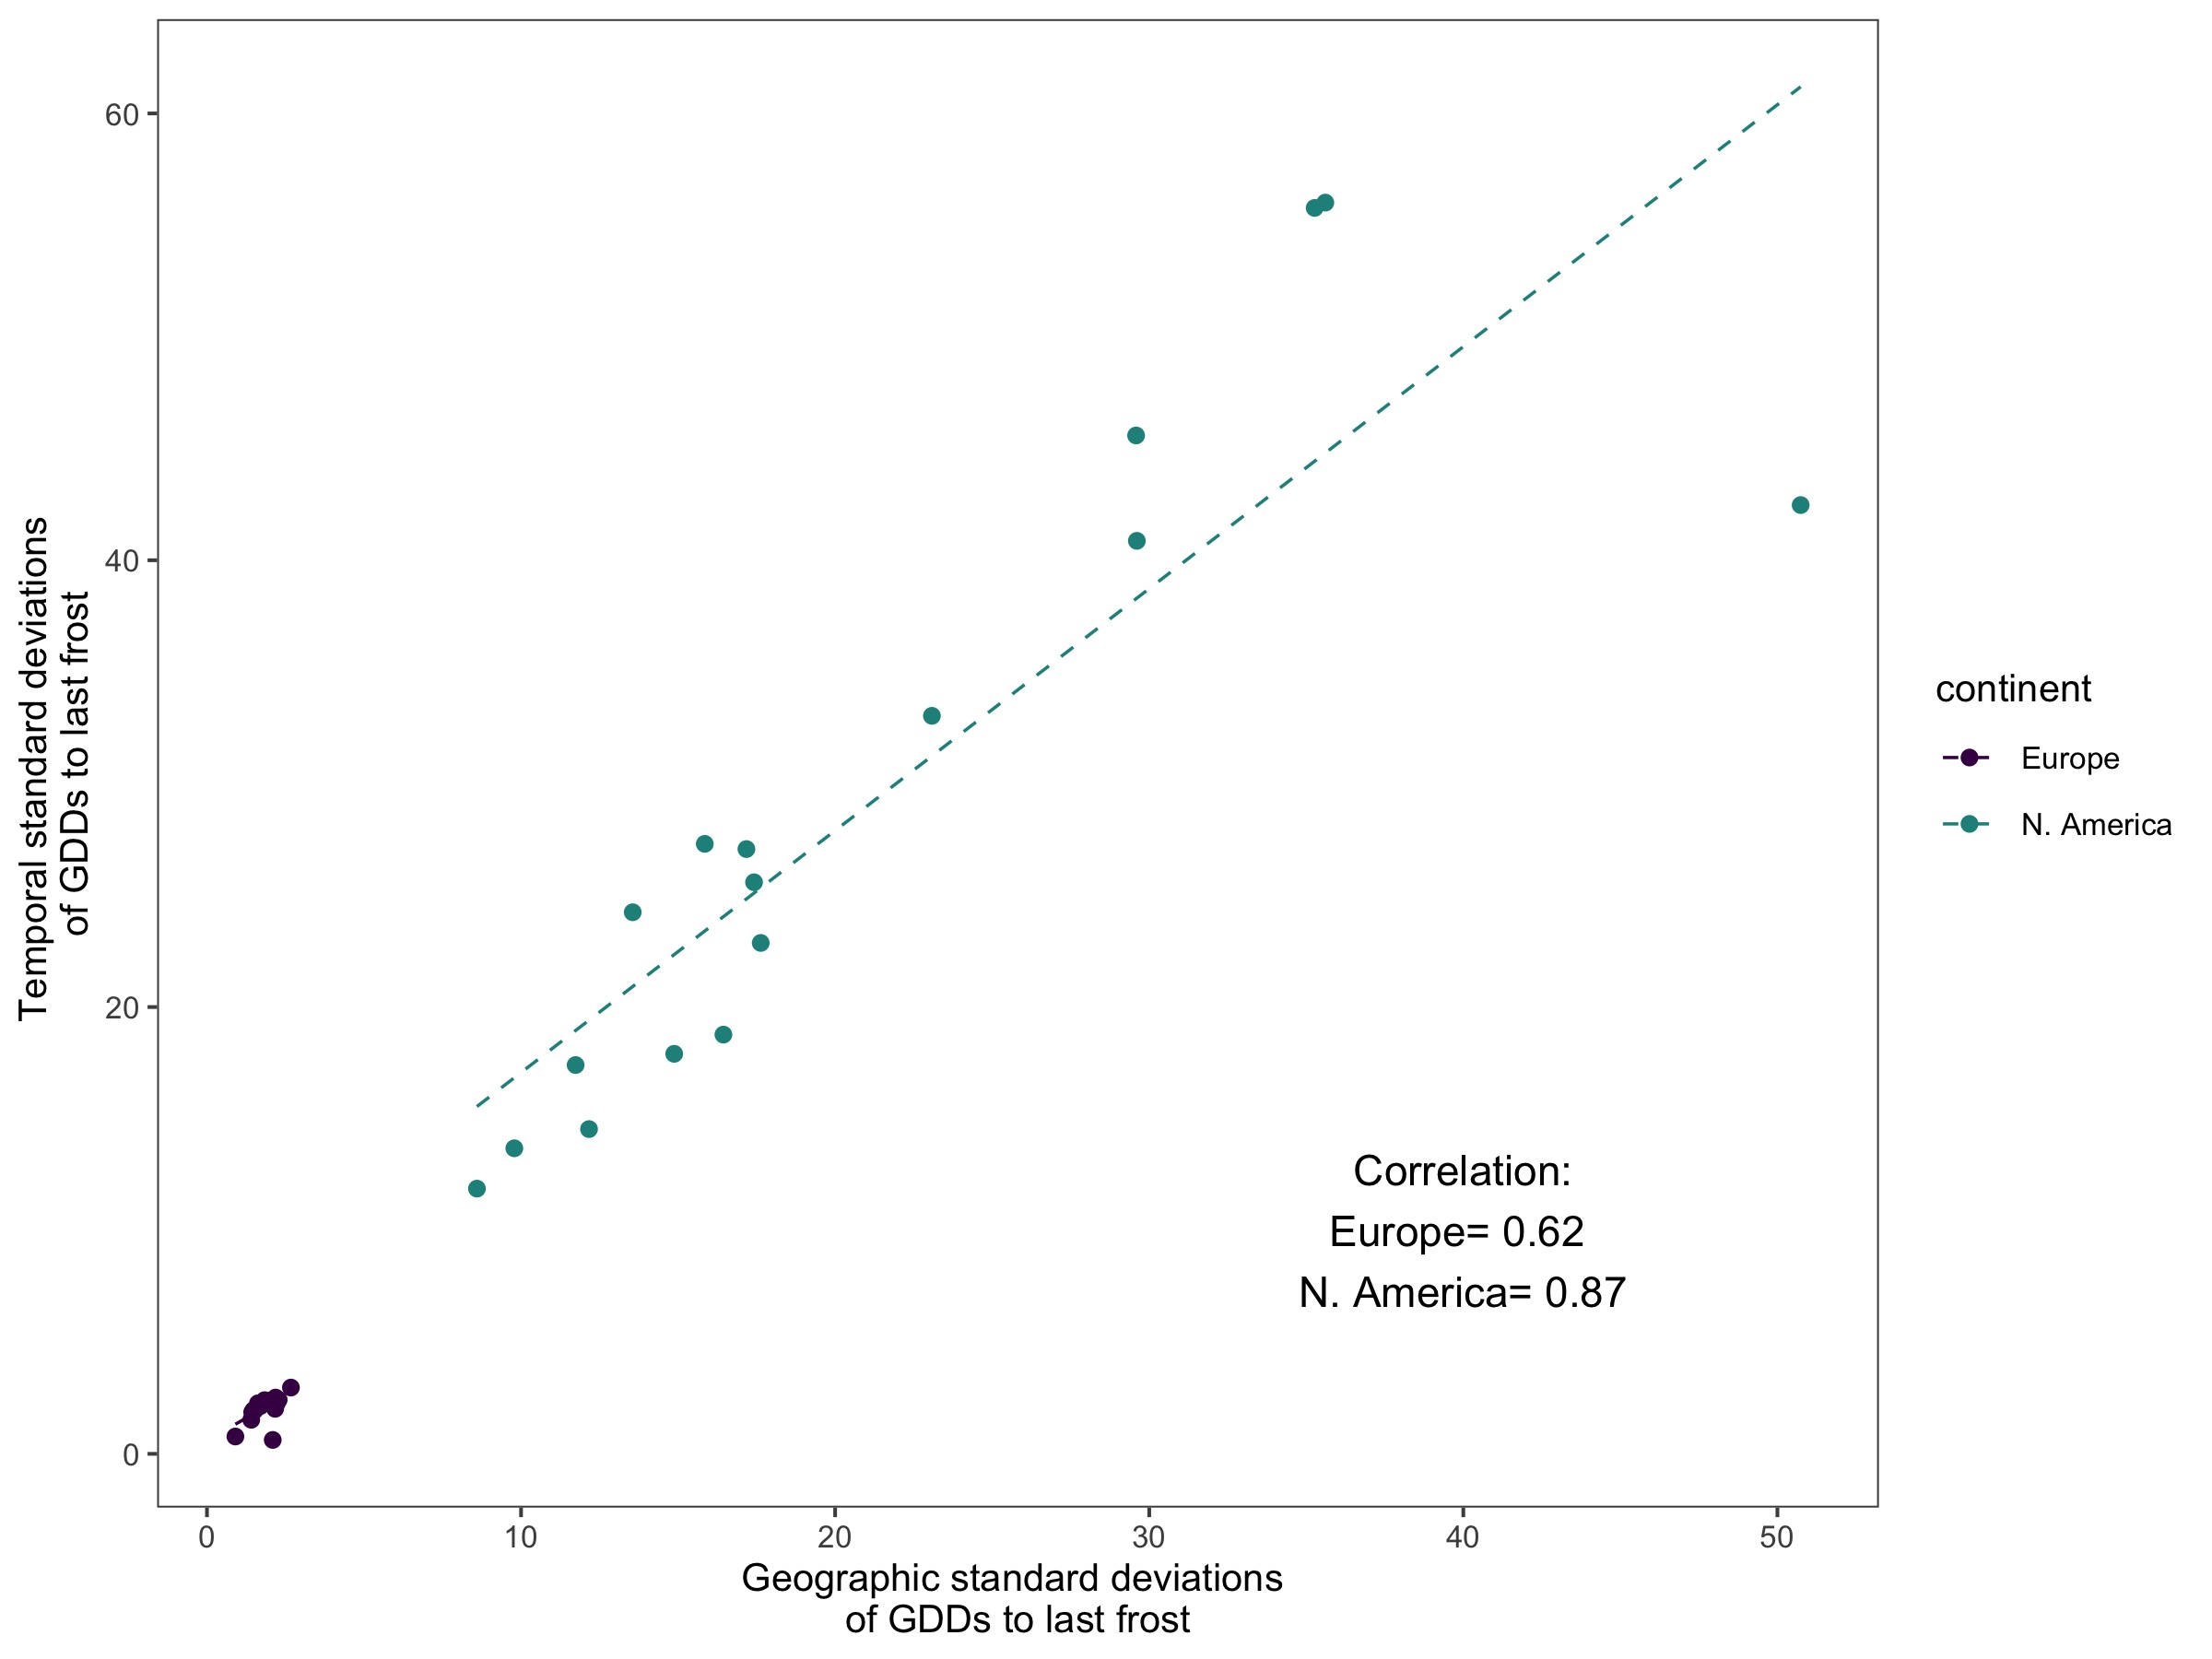
\includegraphics[width=\textwidth]{..//..//analyses/ranges/figures/clim_params.jpeg} 
    \label{fig:corrs}
\end{figure}

\begin{figure}[h!]
    \centering
 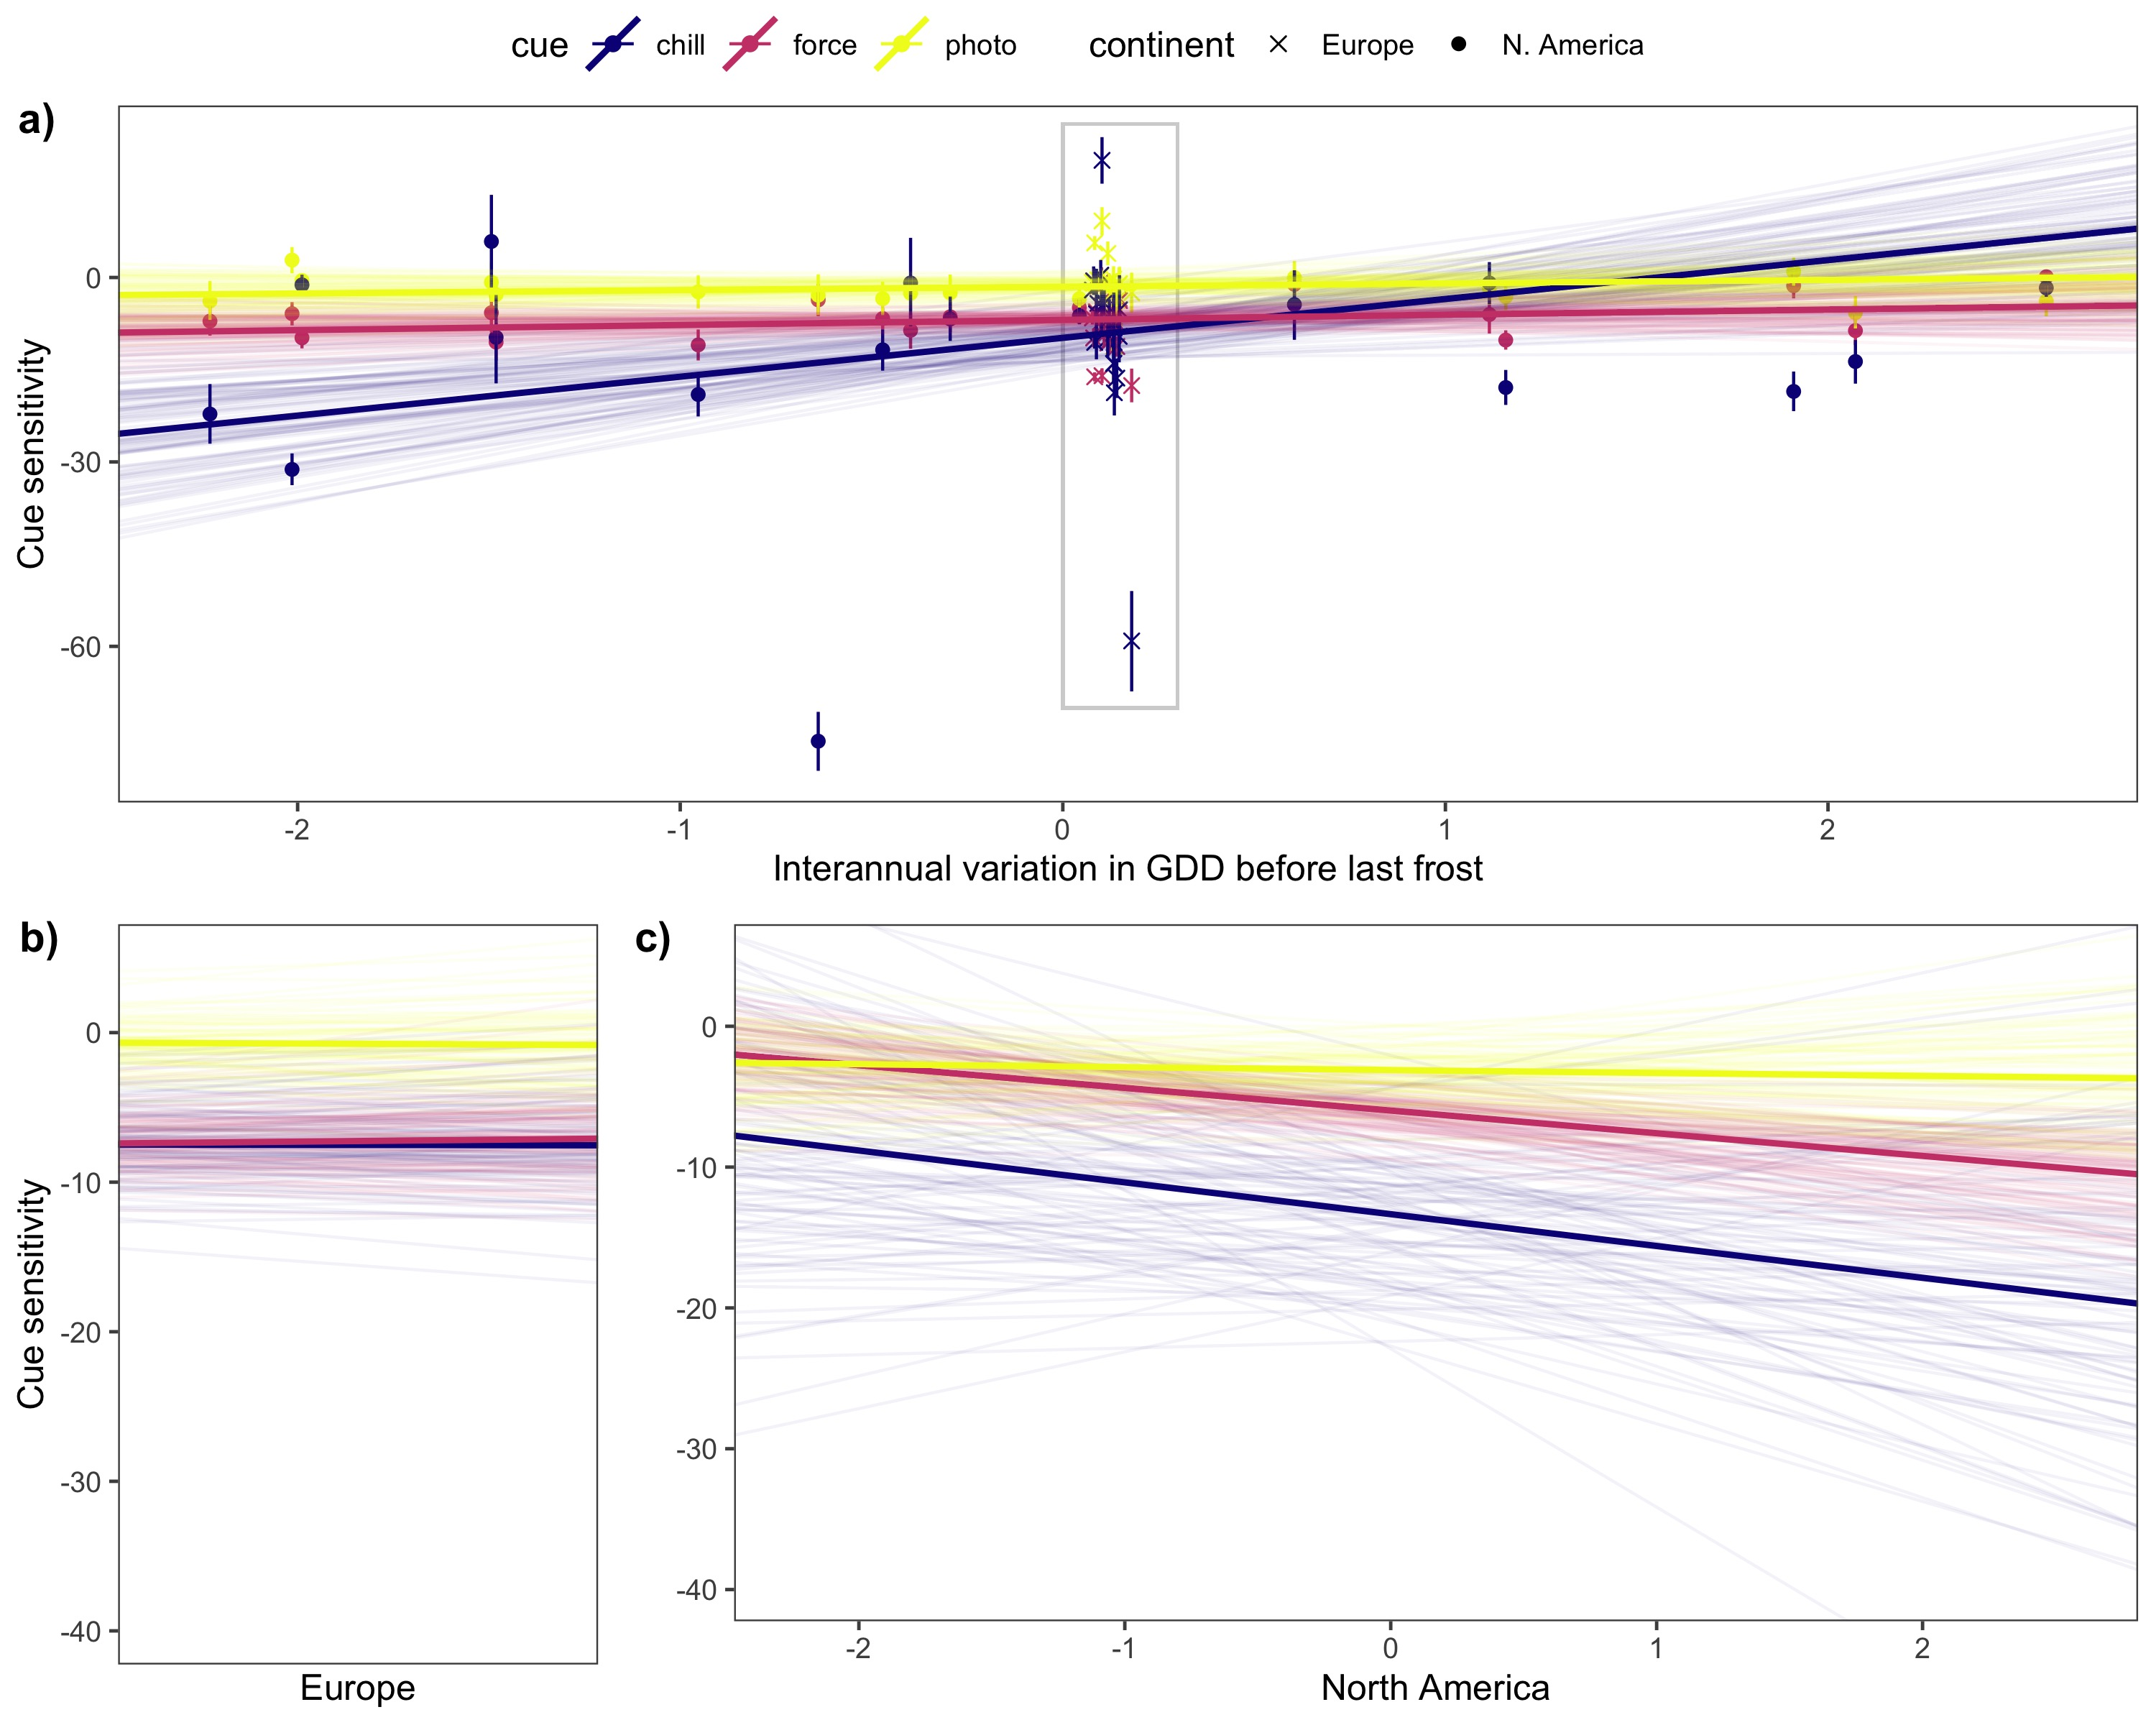
\includegraphics[width=\textwidth]{..//..//analyses/ranges/figures/mock1.jpeg} 
    \caption{ }
    \label{fig:mods2}
\end{figure}

\begin{figure}[h!]
    \centering
 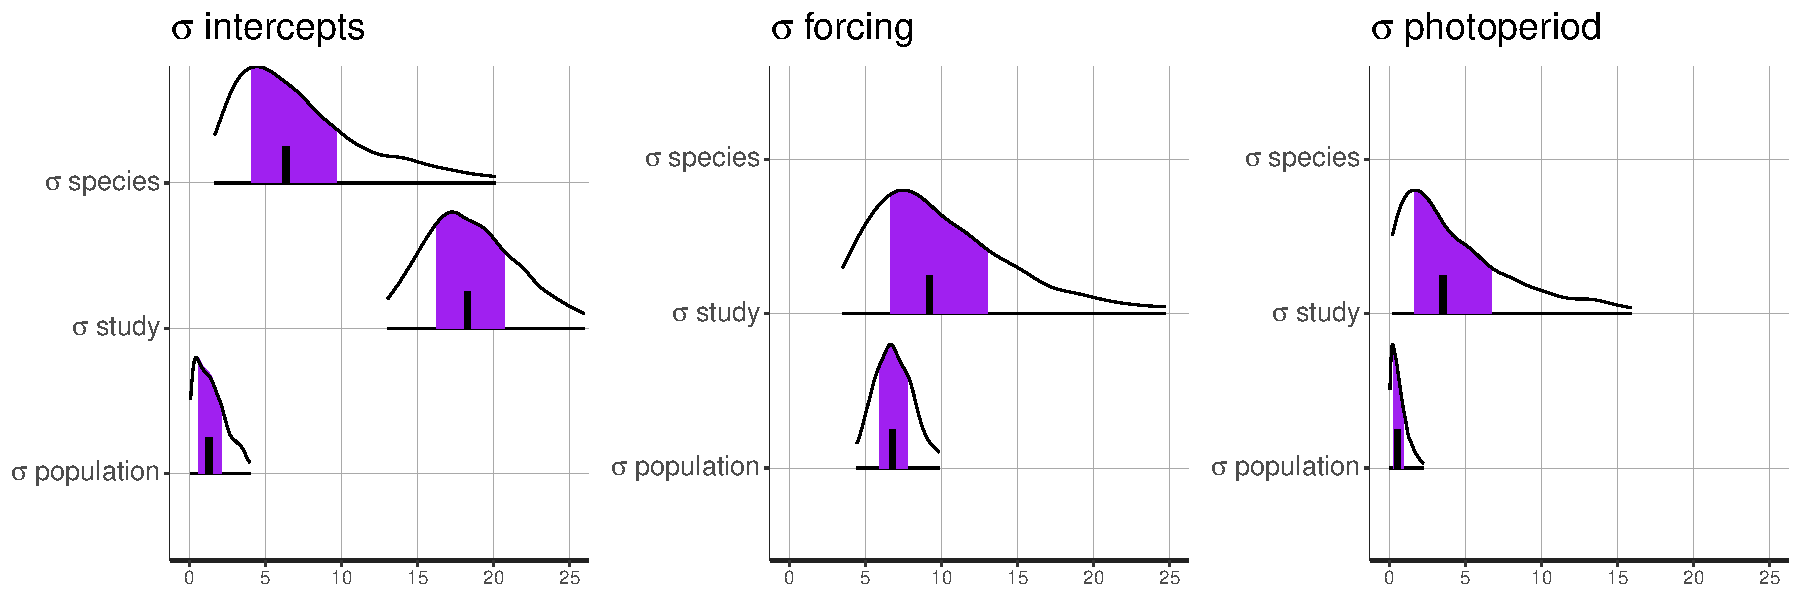
\includegraphics[width=\textwidth]{..//..//analyses/ranges/figures/variancepartitioning.pdf} 
    \caption{ \textbf{Local adaptation model estimates of variation partitioning in the intercept and forcing and photoperiod predictors using the OSPREE dataset}. For both the forcing and photoperiod predictors, within species (intraspecific) variation is much smaller than across species (interspecific) variation. Here we see that interspecific variation exceeds intraspecific variation at the intercept-level as well but variation at the study level is largest, suggesting experimental design is driving the highest level of uncertainty.}
    \label{fig:popy}
\end{figure}






\end{document}

%CJCFeb15: you might be able to cite Fu et al 2015 Nature paper above... it's been a while since I've read it though
%EMWFeb5: A small but important thing missing from the above paragraph is that we need a way to predict these cues across many species (related to ths idea that we don't (or can't) measure these cues for all species ... so we need a predictive framework). It could be something you add at the end of this paragraph?

%\textbf{ But the quantification of cue use difference among species offers even more---a novel opportunity to interrogate long-standing theories regarding the biology underlying cue-use difference among species.} One particular relationship that can now be examined this the relationship species' geographic ranges and phenological cue use.
%EMWFeb5: Adjusted text so we don't say 'widely assumed,' I don't think we need it. 
%Climate is the major selective force on both species' geographic ranges \citep{Morin:2011aa} and their phenology \citep{Savage:2013aa} and, therefore, phenological cue-use differences among species may reflect the climate of their respective ranges \citep{Zohner:2017aa,Silvestro:2019wa}. That is, a species' relative reliance on forcing, chilling and photoperiod should be shaped by the unique environmental conditions across a species' geographic range.
%IMCFeb21: I wondered if we should mention already here that cue-use being reflective of within-range climate would rely on an  assumption of little effects of local adaptation? Also, the environmental conditions can be pretty variable within a range, so perhaps delete 'unique'?  

Despite this intuitive link between climate and cues, direct tests of this assumption are rare (but see \citep{Zohner:2017aa}). With the recent quantification of cue-use differences of many species \citep{Ettinger:2020aa} and the accessibility of high resolution climate data it is now possible to rigorously test this theory with data. Below, we briefly outline two hypotheses about the relationship between phenological cue-use and species' climatic range characteristics, as well as possible complications/complexities (assumptions?) underlying them. We then test these predictions using Bayesian models for a large suite of temperate woody species from North America and Europe.
%EMWFeb5: edits above ... two next paragraphs below are great!

\subsection{Climate intensity hypothesis}
One hypothesis for the evolution of cue-use differences across species is that species utilize the climate cues to which they have the most exposure. Simply stated, there should be a positive correlation between the amount or intensity of a cue across a species' range and the species phenological sensitivity to that cue. This hypothesis predicts that species with  a) high numbers of growing degree days in their range should have stronger forcing cues and b) higher amounts of chilling should have stronger chilling cues.%. and c) more annual photoperiod variation should have stronger photoperiod cues. %This hypothesis has been applied to explain large, macro-ecological patterns in phenology like why the tropical phenology cues primary to forcing and temperate and arctic phenology is more dependent on photoperiod and/or chilling \citep{} but has not been widely tested within biomes for species with overlapping ranges.  
%IMCFeb21: I'd suggest the following edit: This hypothesis predicts that species exposed to ... within their range. 

\subsection{Climate variability hypothesis}

Current understanding of the evolution of phenological cues assume that forcing is the predominant cue. In this framework, a secondary reliance on photoperiod and/or chilling cues evolve when forcing alone is not a reliable cue of safe growing condition \citep{Korner:2010aa}. Forcing is is an unreliable cue when temperatures are unstable in the spring time. The climate variability hypothesis predicts species with high variation in spring temperature in their range should evolve a stronger response to all three cues, especially chilling and or photoperiod \citep{Wang:2014aa, Muffler2016}. 
%This hypothesis potentially explains the stronger cue sensitivity of temperate North American species to those in Europe where there is less climate variability in the spring \citep{Zohner:2017aa}.
%CJCFeb15: does this same hypothesis not apply to climate variability in the winter? So if chilling cues are less reliable?
%IMCFeb21: Perhaps change 'evolution of phenological cues' for 'relative importance or effects of phenological cues' 

%EMWFeb5: I both (1) think this is impt enough for intro/discussion and (2) don't think this will work in methods that easily. I suggest a new subheader: Complexities: Spatio-temporal variability and population-level effects ... or maybe better: Assumptions: Spatio-temporal coherency and small population-level effects 
\textbf{I want to move the following paragraph to de-emphysize this point. I am thinking maybe somewhere in the methods.} However, a major hurdle to robustly testing this hypothesis is that, when considered in the context of a species' geographic range, spring temperature variation occurs on multiple temporal and spatial scales. Phenology may be shaped by intra-annual temperature variation (e.g. frequency of late season frost, diurnal temperature functions), inter-annual variation (e.g. annual mean temperatures) and the interaction between them (e.g. inter-annual variation in last season frost episodes). Further, each of the level of variation be quite different across a species range, suggesting geographic variation with the range must also be accounted for. %CJCFeb15: Suggested edits to this sentence... "Further, geographic variation within a species' range can be quite different and must be accounted for." And then start the next sentence with... "Geographic variation could drive selection for secondary cue usage (photoperiod/chilling), and it is unclear how the two interact or which is important"
Any of these levels of variation could itself drive selection for secondary cue usage (photoperiod/chilling), and it is unclear how they interact or which is most important \citep{Zagmajster:2014aa}. Key to testing the climate variability hypotheses is to first characterize relationships between spring temperature variation at multiple spatio-temporal scales because ... %EMWFeb5: Spell out why this matters.
%CJCFeb15: These species that are more `flexible' in cue use (i.e., species with greater geographic variation and ability to rely on secondary cue use), would this suggest greater flexibility in range shifts with climate change? Or this idea of phenological tracking? I'm not sure this is an important piece to dive in here but maybe we can set it up for the discussion if you agree with this hypothesis.
%IMCFeb21: This is a terminological comment so if you don't agree please ignore. I'm not sure the emphasis should so much be on the 'scale' because we don't really look at different scales (we have one temporal scale: year, and one spatial scale per continent). So I wondered if we should emphasize more the fact that there is wide spatial-temporal variation (i.e. climate can differ a lot in one single location across years and across multiple locations in one single year)  

\noindent An implicit assumption of the previously stated hypotheses is that among species cue-use variation is higher than within species (i.e. cue use is ``conserved" at the species level). If rather, cue use patterns are locally adapted, while climate intensity and climate variability may still drive cue-use patterns at the population level, it would be difficult to detect consistent patterns across a species full geographic range. There is not yet a strong consensus about to what degree cue-use is locally adapted and it likely varies between phenophases and organisms \citep{Vitasse2010,,}. As such, any analysis considering species ranges and cue use must account for intra-specific differences as well.
